\documentclass[aps,pre,reprint,amsmath,amssymb,longbibliography]{revtex4-2}
\usepackage{graphicx}
\usepackage{booktabs}
\usepackage{xr-hyper}
\usepackage{hyperref}
\hypersetup{colorlinks=true,linkcolor=blue,citecolor=blue,urlcolor=blue}
% Keep title line breaks out of PDF metadata.
\pdfstringdefDisableCommands{\def\\{ }}
% Tectonic's XeTeX driver needs exported destination names for cross-PDF links.
% Scope remote-link state to avoid hyperref issue latex3/hyperref#107.
\makeatletter
\@ifundefined{XeTeXversion}{}{%
  \let\paper@linkfile\hyper@linkfile
  \def\hyper@linkfile#1#2#3{%
    \begingroup\paper@linkfile{#1}{#2}{#3}\endgroup}
  \AtBeginDvi{\special{dvipdfmx:config C 0x10}}
}
\makeatother
\graphicspath{{../figures/nucleation/paper/}}
\renewcommand{\dbltopfraction}{0.95}
\renewcommand{\topfraction}{0.95}
\renewcommand{\textfraction}{0.05}
\renewcommand{\floatpagefraction}{0.8}
\renewcommand{\dblfloatpagefraction}{0.8}

\makeatletter
\newenvironment{appendixfigure}
  {\par\addvspace{8pt}\noindent\begin{minipage}{\textwidth}\def\@captype{figure}\centering}
  {\end{minipage}\par\addvspace{10pt}}
\makeatother
% Shared notation is defined in the manuscript.
\newcommand{\RR}{\mathbb{R}}

% Generated from the complete analysis referenced by phase_inputs.json.
\newcommand{\PhaseBPoints}{41}
\newcommand{\PhaseDPoints}{41}
\newcommand{\PhaseRuns}{215168}
\newcommand{\CompactA}{29}
\newcommand{\CompactB}{0}
\newcommand{\CompactU}{35}
\newcommand{\RandomA}{1}
\newcommand{\RandomB}{39}
\newcommand{\RandomU}{24}


% Shared title and author metadata for the article and Supplemental Material.
\newcommand{\papertitle}{Stochastic collapse of spatial cooperation:\\Perturbation geometry and resource alignment}
\newcommand{\paperauthorblock}{%
\author{Bingkun Zhao}
\email{bingkzhao2-c@my.cityu.edu.hk}
\affiliation{Hong Kong Institute of AI for Science, City University of Hong Kong, Hong Kong SAR, China}
\author{Xie Li}
\email{xieli@zzu.edu.cn}
\affiliation{School of Management, Zhengzhou University, Zhengzhou, Henan, China}
\thanks{Corresponding author: xieli@zzu.edu.cn}
}
\hypersetup{pdfauthor={Bingkun Zhao, Xie Li}}

\externaldocument[main-]{main}
\renewcommand{\thesection}{S\Roman{section}}
\renewcommand{\theequation}{S\arabic{equation}}
\renewcommand{\thefigure}{S\arabic{figure}}
\renewcommand{\thetable}{S\arabic{table}}
\renewcommand{\bibnumfmt}[1]{[S#1]}
\renewcommand{\citenumfont}[1]{S#1}
\begin{document}
\raggedbottom
\title{Supplemental Material for\\\papertitle}
\paperauthorblock
\maketitle
\noindent
This document contains complete derivations, numerical protocols, additional
controls, and supporting spatial and dynamical results. Figures, equations,
tables, sections, and literature citations belonging to this document carry
an S prefix; unprefixed numbers refer to the main article.
\section{Mathematical derivations}
\label{sec:proofs}

\subsection{First-visit law and exponent clipping}

Fix a strategy field and the resource field used for imitation. A cooperator copying a defector contributes $+1$ to the defector increment $Z$; the reverse copying event contributes $-1$. All other visits contribute zero. Uniform selection of the first site and its neighbor gives
\begin{equation}
\label{eq:probabilities}
p_+=\frac{1}{4N}\sum_{e\in\mathcal I}F(x_e),
\qquad
p_-=\frac{1}{4N}\sum_{e\in\mathcal I}F(-x_e).
\end{equation}
An undirected interface edge can be sampled in either orientation, each with probability $1/(4N)$ during the first visit. All other visits leave the defector count unchanged. The remaining probability is $1-p_+-p_-$; it is nonnegative because the square lattice has at most $2N$ undirected edges and $p_++p_-=P/(4N)\le1/2$. The relations below follow from the symmetry of the smooth Fermi rule and concern the single visit conditioned on the initial configuration.

To prove complementarity, write $F(x)=e^x/(1+e^x)$ and $F(-x)=1/(1+e^x)$. Their sum is one. Expressing the hyperbolic functions through exponentials also gives $2F(x)-1=\tanh(x/2)$. Substituting into Eq.~\eqref{eq:probabilities} yields $p_+-p_-=J/N$ and $p_++p_-=P/(4N)$. Since $Z\in\{-1,0,1\}$, its mean is $p_+-p_-$ and its second moment is $p_++p_-$. Subtracting the squared mean proves the variance in Eq.~\eqref{main-eq:moments}.

Moreover, $0<F(x)<1$ implies $|2F(x)-1|\le1$. The finite-sum triangle inequality gives
\begin{equation}
\label{eq:drift_bound}
|J|\le\frac14\sum_{e\in\mathcal I}|2F(x_e)-1|
\le\frac P4.
\end{equation}
When $P=0$, all three first-visit moments vanish. These statements require no independence between successive visits: they describe one visit conditioned on its initial state.

For the numerical clipping convention, define $c_M(x)=\max\{-M,\min(M,x)\}$ with $M=30$. It obeys $c_M(-x)=-c_M(x)$, including at the clipping endpoints. Thus $F(c_M(x))+F(c_M(-x))=1$, and the same second-moment identity holds exactly. The exact clipped mean uses
\begin{equation}
\label{eq:clipped}
J^{(M)}=\frac14\sum_{e\in\mathcal I}
\tanh[c_M(x_e)/2]
\end{equation}
in place of the smooth $J$. The identities for the clipped mean use $J^{(M)}$, whereas the smooth diagnostic $J$ is used for the sensitivity derivatives and reported interface-bias plots. These statements are algebraic properties of the clipping convention; they do not equate exact real arithmetic with floating-point simulation behavior.

\subsection{Initial interface geometry}

Immediately after seeding, every cooperator has resource one and every defector has resource zero. The local reaction leaves these values unchanged. If a boundary cooperator has $a$ cooperative neighbors, its resource after diffusion is
\begin{equation}
\label{eq:initial_resource}
r_C^+=1-\frac D4(4-a).
\end{equation}
Consider a neighboring defector with $c$ cooperative neighbors. The initial payoff difference on this edge is therefore
\begin{equation}
\label{eq:initial_gap}
\Pi_D-\Pi_C
=bc-a\!\left[1+\lambda\sigma
 \left(1-\frac D2(4-a)\right)\right]
\end{equation}
on the positive reward branch. Let $H_{ac}$ count interface edges having these two neighbor counts, where $0\le a\le3$ and $1\le c\le4$. Grouping the interface sum gives
\begin{equation}
\label{eq:motifs}
J_{\rm pre}(0)=\frac14
\sum_{a=0}^{3}\sum_{c=1}^{4}
H_{ac}\tanh\!\left[\frac{\Pi_D(c)-\Pi_C(a)}{2K}\right].
\end{equation}
For an isolated defector, $H_{3,4}=4$ and all other counts vanish. Substitution proves Eq.~\eqref{main-eq:isolated}. Its zero-bias temptation is
\begin{equation}
\label{eq:isolated_zero}
b_0(D)=\frac34[1+\lambda\sigma(1-D/2)].
\end{equation}
At the reference coupling, this is $1.125-0.1875D$. It is an initial local payoff balance, not a predicted depletion threshold. Multiple seeds can alter one another's neighbor counts and resource environments, which is why the measured $H_{ac}$ rather than $m$ controls their initial interface bias.

\subsection{Total resource balance and diffusion modes}

Define $u_i$ by Eq.~\eqref{main-eq:resource}. Every site appears four times in the nearest-neighbor sum on the periodic lattice. Hence
\begin{equation}
\label{eq:resource_total}
\sum_i r_i^+
=(1-D)\sum_i u_i+\frac D4\sum_i\sum_{j\sim i}u_j
=\sum_i u_i.
\end{equation}
Expanding the local increment yields
\begin{equation}
\label{eq:local_balance}
u_i-r_i=g s_i-\delta r_i+(\delta-g)s_i r_i.
\end{equation}
Summation and division by $N>0$ give the first line of Eq.~\eqref{main-eq:balance}. Substituting $\langle sr\rangle=\rho\bar r+C_{sr}$ and collecting terms proves the covariance form. This derivation retains the spatial correlation exactly. Dropping $C_{sr}$ would be an additional closure assumption.

For a fixed set of sites $\Omega$, the same calculation separates local reaction from transport:
\begin{equation}
\label{eq:flux}
\sum_{i\in\Omega}(r_i^+-u_i)
=\frac D4
\sum_{\substack{i\in\Omega,\ j\notin\Omega\\j\sim i}}
(u_j-u_i).
\end{equation}
To obtain this expression, write each diffusion increment as $(D/4)\sum_{j\sim i}(u_j-u_i)$. For an internal pair $i,j\in\Omega$, the two terms are opposite and cancel. Only boundary-crossing pairs remain. The formula concerns a fixed region during the resource substep; a moving strategy domain has additional membership changes. We do not infer a measured front velocity or a flux-controlled growth law from this identity.

For pure diffusion, a lattice Fourier mode with wave vector $(k_x,k_y)$ has multiplier
\begin{equation}
\label{eq:diffusion_mode}
\Lambda_D(k_x,k_y)=
1-D+\frac D2(\cos k_x+\cos k_y),
\end{equation}
with $k_\alpha=2\pi n_\alpha/L$. Each pair of opposite translations contributes $2\cos k_\alpha$ times the mode, giving Eq.~\eqref{eq:diffusion_mode}. The same relation follows for separable real sine and cosine modes by the angle-addition identities. Since each cosine lies in $[-1,1]$,
\begin{equation}
\label{eq:mode_bound}
1-2D\le\Lambda_D\le1,
\qquad |\Lambda_D|\le1.
\end{equation}
For even $L$, the checkerboard mode has multiplier $1-2D$, which is negative when $D>1/2$. Diffusion can therefore reverse a mode's sign without increasing its magnitude. For perturbations about a homogeneous resource equilibrium, local reaction multiplies this factor by $1-g$ in an all-cooperator field or by $1-\delta$ in an all-defector field. For a nonuniform strategy pattern, multiplication by $A_s$ mixes the Fourier modes. A single diffusion eigenvalue does not determine the duration of a resource intervention in the coupled system.

\subsection{Existence, uniqueness, and accuracy of the adapted field}

For fixed $s$, the local maps are $f_C(r)=(1-g)r+g$ and $f_D(r)=(1-\delta)r$. If $r\in[0,1]$ and $0\le g,\delta\le1$, both maps remain in $[0,1]$. Diffusion is a convex average, so $T_s$ maps the closed cube $[0,1]^N$ into itself.

For two fields, the local differences satisfy $|f_{s_i}(r_i)-f_{s_i}(\widetilde r_i)|\le q|r_i-\widetilde r_i|$, where $q=\max\{1-g,1-\delta\}$. Nonnegative averaging weights with unit row sum give
\begin{equation}
\label{eq:average}
\begin{aligned}
|T_s(r)_i-T_s(\widetilde r)_i|
&\le\sum_j (M_D)_{ij}q|r_j-\widetilde r_j|\\
&\le q\|r-\widetilde r\|_\infty.
\end{aligned}
\end{equation}
Taking the maximum and applying induction proves Eq.~\eqref{main-eq:contraction}.

If $0<g,\delta\le1$, then $q<1$. Starting from any $r^{(0)}$ in the cube, set $r^{(n+1)}=T_s(r^{(n)})$. Consecutive differences obey
\begin{equation}
\label{eq:iterate_gap}
\|r^{(n+1)}-r^{(n)}\|_\infty
\le q^n\|r^{(1)}-r^{(0)}\|_\infty.
\end{equation}
For $m>n$, sum these differences to obtain
\begin{equation}
\label{eq:cauchy}
\|r^{(m)}-r^{(n)}\|_\infty
\le\frac{q^n}{1-q}\|r^{(1)}-r^{(0)}\|_\infty.
\end{equation}
The finite-dimensional real space is complete, so the sequence converges. The cube is closed, hence its limit belongs to the cube. Continuity of $T_s$ makes the limit a fixed point. Two fixed points at distance $d$ satisfy $d\le qd$, forcing $d=0$. This proves existence, uniqueness, and convergence to the physical adapted field through the Banach contraction theorem.

The affine form also displays the equilibrium equation explicitly:
\begin{equation}
\label{eq:equilibrium_linear}
(I-M_DA_s)r_{\rm eq}=gM_Ds.
\end{equation}
Since $\|M_DA_s\|_\infty\le q<1$, its inverse can be represented by the convergent geometric operator series. This is an alternative expression for the same fixed point, not a separate physical approximation.

For any trial field $r$, the triangle inequality and contraction give
\begin{equation}
\label{eq:residual_proof}
\begin{aligned}
\|r-r_{\rm eq}\|_\infty
&\le\|r-T_s(r)\|_\infty
  +\|T_s(r)-T_s(r_{\rm eq})\|_\infty\\
&\le\|r-T_s(r)\|_\infty+q\|r-r_{\rm eq}\|_\infty.
\end{aligned}
\end{equation}
Rearranging proves Eq.~\eqref{main-eq:equilibrium_error}. If an iteration stops when $\|r^{(n+1)}-r^{(n)}\|_\infty\le\varepsilon$ and returns the new iterate, one further use of contraction gives
\begin{equation}
\label{eq:returned_error}
\|r^{(n+1)}-r_{\rm eq}\|_\infty
\le\frac{q}{1-q}\varepsilon.
\end{equation}
For $q=0.9$ and a stopping tolerance of $10^{-13}$, the real-arithmetic returned-iterate bound is $9\times10^{-13}$, provided termination occurs by the tolerance criterion. The implementation also imposes a 500-step cap; reaching that cap alone does not certify the same accuracy. These bounds do not account for floating-point roundoff.

The diagnostics $\eta$ and $J_{\rm eq}$ in Eq.~\eqref{main-eq:adaptation} use this fixed-strategy field. In the coupled system, both $s$ and its equilibrium field change. Their definitions do not imply that $\eta$ or $J-J_{\rm eq}$ is a sufficient coordinate for future depletion.

\subsection{Sensitivity through the resource substep}

For one interface edge incident on a boundary cooperator $u$, write
\begin{equation}
\label{eq:edge_derivative}
J_e=\frac14\tanh z_{uv},
\qquad
\frac{\partial z_{uv}}{\partial r_u}
=-\frac{\lambda\sigma k_C(u)}{K}.
\end{equation}
On the positive reward branch, $R'=2\lambda\sigma$. Applying the derivative $(\tanh z)'=1-\tanh^2z$ and summing all incident defector edges proves Eq.~\eqref{main-eq:sensitivity}. The strategy pattern and neighbor counts are held fixed. A defector's own resource does not enter its payoff, so its direct derivative in $J(s,r)$ vanishes.

The intervention is applied to $r$, whereas imitation uses $T_s(r)$. For a direction $h$, the affine resource map gives the exact variation
\begin{equation}
\label{eq:resource_variation}
T_s(r+\epsilon h)-T_s(r)=\epsilon M_DA_sh.
\end{equation}
At a smooth reference point, the chain rule yields
\begin{equation}
\label{eq:chain}
\begin{aligned}
\left.\frac{d}{d\epsilon}J(s,T_s(r+\epsilon h))\right|_0
&=-w^\mathsf{T}M_DA_sh\\
&=-\sum_u a_u(M_D^\mathsf{T}w)_u h_u.
\end{aligned}
\end{equation}
The second line follows by exchanging the finite sums; it does not require independent resources. Symmetry of periodic nearest-neighbor diffusion gives $M_D^\mathsf{T}=M_D$, producing $W_u$ in Eq.~\eqref{main-eq:effective_weight}. The Taylor remainder is quadratic in the maximum norm, for fixed $N$, strategies, and model parameters with $K>0$, along perturbations whose entire segment remains on the positive reward branch. Indeed, $|\tanh''z|\le2$ bounds the remainder of an edge contribution by $(\Delta z_{uv})^2/4$. Convex diffusion and the local slopes give $|\Delta z_{uv}|\le |\lambda\sigma|k_C(u)q\|h\|_\infty/K$. Summing over the fixed interface proves the stated order, with a constant no larger than $9P(\lambda\sigma)^2q^2/(4K^2)$ because a boundary cooperator has at most three cooperative neighbors. This constant is not uniform as $K\to0$ or the interface grows. Finite permutations are evaluated with the nonlinear expression.

This derivation also explains why moving resource among defectors can affect the next strategy-update cycle. Their direct weights $w_u$ vanish, but a neighboring boundary cooperator can contribute to $W_u$ through diffusion. There is no general geometry-independent ratio between the two intervention responses.

\subsection{Rearrangement inequality and invariants}

Let $\mathcal B$ be the fixed set of boundary cooperators. On this set, $a_u=1-g$ is common, so maximizing the linear protective response amounts to maximizing $\sum_{u\in\mathcal B}W_u r_{\pi(u)}$ over permutations $\pi$. Order the weights as $W_1\le\cdots\le W_m$ and the resource values as $r_1\le\cdots\le r_m$. The rearrangement inequality states
\begin{equation}
\label{eq:rearrangement}
\sum_{i=1}^m W_i r_{m+1-i}
\le \sum_{i=1}^m W_i r_{\pi(i)}
\le \sum_{i=1}^m W_i r_i.
\end{equation}
For completeness, consider two weights $W_i\le W_j$ and values $r_i\le r_j$. The gain from aligning their orders is
\begin{equation}
\label{eq:exchange}
(W_i r_i+W_j r_j)-(W_i r_j+W_j r_i)
=(W_j-W_i)(r_j-r_i)\ge0.
\end{equation}
Whenever an assignment is not ordered, exchanging an inverted pair cannot decrease the objective. Repeated exchanges reach the same-order assignment in finitely many steps, proving the upper bound. Reversing the ordering proves the lower bound. Ties yield zero exchange gain and do not change the result.

For any function $\phi$ of a resource value, bijectivity of $\pi$ gives
\begin{equation}
\label{eq:permutation}
\sum_{u\in\mathcal B}\phi(r_{\pi(u)})
=\sum_{u\in\mathcal B}\phi(r_u).
\end{equation}
Taking $\phi(r)=r$ proves preservation of the boundary total and mean. Taking indicator functions proves preservation of the empirical resource distribution. Sites outside $\mathcal B$ are unchanged, so the global distribution and total are also preserved. The nonnegative factor $1-g$ retains the ordering of the linear objective; at $g=1$ it vanishes. The full nonlinear $J_{\rm pre}$ and the continuation fate need not share these extrema.

\subsection{Translation preserves resource autocorrelation}

On the finite periodic lattice, the map $i\mapsto i-\mathbf d$ is a bijection and commutes with every other translation. Since it also preserves the spatial mean, the autocorrelation of a translated field is
\begin{equation}
\label{eq:translation_autocorrelation_proof}
\begin{aligned}
\Gamma_{\mathcal T_{\mathbf d}r}(\mathbf a)
&=\frac1N\sum_i(r_{i-\mathbf d}-\bar r)
                  (r_{i+\mathbf a-\mathbf d}-\bar r)\\
&=\frac1N\sum_j(r_j-\bar r)(r_{j+\mathbf a}-\bar r)
=\Gamma_r(\mathbf a).
\end{aligned}
\end{equation}
The substitution $j=i-\mathbf d$ proves the result at every lag. The covariance with an untranslated strategy field has no analogous invariance, because the strategy factor changes under the same reindexing.

\subsection{Cumulative response and finite event counts}

The cumulative relation in Eq.~\eqref{main-eq:cumulative_response} follows by summing consecutive differences of $\mathbb E_a[n_D(u)]-\mathbb E_0[n_D(u)]$. Interior terms cancel and the initial term vanishes because the strategies initially coincide. Since $0\le n_D\le N$ and the sum is finite, expectation and summation commute without an independence assumption.

For the empirical reach decomposition, let $\mathcal B_T$ and $\mathcal R_T$ contain the realizations that collapse and reach the selected population threshold by $T$. Here $\mathcal B_T\subseteq\mathcal R_T$. Multiplying the reaching fraction by the conditional collapse fraction cancels $|\mathcal R_T|$, provided this count is positive, proving the sample counterpart of Eq.~\eqref{main-eq:reach_decomposition}. The two reported reaching counts are nonzero. Similarly, the eventual collapsed set contains $\mathcal B_T$ and is contained in $\mathcal B_T\cup\mathcal U_T$. Monotonicity of finite cardinality gives Eq.~\eqref{eq:unresolved_bound}.

Subtracting the two resource balances with equal initial $\rho$ and $\bar r$ proves Eq.~\eqref{main-eq:translation_balance}. Solving the same balance for $C_{sr}$ when $\delta\ne g$ proves Eq.~\eqref{eq:reconstruct_covariance}.

\section{Numerical methods and supplementary controls}
\label{sec:checks}

\subsection{Event clocks and continuation probabilities}

Let $I_t=\mathbf 1\{\rho(t)\le0.2,\ \bar r(t)\le0.2\}$ and let $c_t$ count consecutive MCS inside this joint threshold:
\begin{equation}
\label{eq:clock}
c_t=
\begin{cases}
c_{t-1}+1,& I_t=1,\\
0,& I_t=0.
\end{cases}
\end{equation}
For a newly perturbed trajectory $c_0=0$. Define $\tau_B=\inf\{t:c_t\ge250\}$ and $\tau_A=\inf\{t:\rho(t)=1,\ \bar r(t)\ge0.6\}$. The first event label is retained. Saved states include both fields, the counter, and any recorded label; the selected configurations have zero counters and no events.

The conditional fate probabilities are defined in main-text Eq.~\eqref{main-eq:conditional_fate}. Times are measured from the continuation origin, unlike $P_\alpha(T)$ and the reach-conditioned factor in Eq.~\eqref{main-eq:reach_decomposition}, which use a common absolute horizon.

For $M$ continuations, the estimates are $\widehat q_\alpha=M_\alpha/M$. If the remaining unresolved paths are eventually assigned either to depletion or to no depletion, their eventual event fraction lies in
\begin{equation}
\label{eq:unresolved_bound}
\frac{M_B}{M}\le \widehat q_{B,\mathrm{eventual}}
\le\frac{M_B+M_U}{M}.
\end{equation}
This interval is a deterministic bound obtained by assigning every unresolved trajectory to one or the other eventual outcome. It is not a confidence interval, and it does not assume that the threshold-defined depletion event is absorbing. Subtracting opposite endpoints for two samples gives $[31/64,41/64]$ for dispersed minus compact in Fig.~\ref{fig:kinetics}.

Figure~\ref{fig:outcomes} gives the complementary recovery and unresolved maps; every cell satisfies Eq.~\eqref{main-eq:partition}. Figure~\ref{fig:sections} resolves all three probabilities at three diffusion strengths.

\subsection{Absorption and stopping}

Without mutation, copying neighbors preserves the all-cooperator state. Diffusion conserves resources, while renewal gives
\begin{equation}
\label{eq:absorbing}
\bar r^+-\bar r=g(1-\bar r)\ge0.
\end{equation}
Once $\bar r\ge0.6$, recovery persists and depletion is excluded. Stopping preserves the event label. Snapshot times record actual execution; the observation horizon remains $T$.

No corresponding proof makes the threshold-defined $B$ set absorbing. A separate persistence check continues 36 confirmed states, one per treatment from each of 12 distinct configurations under original, short-shift, and long-shift protocols. Four new 3000-MCS continuations are generated per state. None of the 144 continuations exceeds cooperation 0.2, and the maximum observed value is 0.1519. These continuations are nested within states and configurations and establish persistence only over that extra window.

\subsection{Finite-window drift and fluctuations}

To follow the response beyond one visit, define the conditional moments from a configuration $X$,
\begin{equation}
\label{eq:finite_moments}
\begin{aligned}
a_\Delta(X)&=\frac{\mathbb E[n_D(\Delta)-n_D(0)\mid X]}{\Delta},\\
b_\Delta(X)&=\frac{\operatorname{Var}[n_D(\Delta)-n_D(0)\mid X]}{\Delta}.
\end{aligned}
\end{equation}
These moments include all updates over $\Delta$ MCS, unlike Eq.~\eqref{main-eq:moments}. Their units are defectors per MCS and defectors squared per MCS. For $x=n_D/N$, they become $a_\Delta/N$ and $b_\Delta/N^2$. The variance rate $b_\Delta$ differs from the payoff parameter $b$.

Figure~\ref{fig:windows} compares original, fixed-strategy-adapted, and translated $(17,12)$ resource fields on the same strategy configurations. Adaptation generally changes the total resource, whereas translation preserves its distribution and total.

Original and adapted fields give similar finite-window moments. At $\Delta=1$, translation changes the mean drift from $-3.89$ to $-15.12$ for compact origins and from $-5.04$ to $-20.02$ for dispersed origins. This difference weakens but persists through $\Delta=20$. The conditional variance rate also decreases with the observation window, with weaker separation between treatments. These scale-dependent moments do not support a constant-coefficient drift--diffusion closure.

\subsection{Spatial selection and conditional-moment estimates}

Figure~\ref{main-fig:fields} uses the smallest seed among confirmed-$B$ trajectories per ensemble, translated once using the initial perturbation center. These are successful examples; threshold statistics use every reaching trajectory.

For the finite-window response in Fig.~\ref{fig:windows}, each configuration contributes $M=64$ independent fresh continuations for each resource treatment. If $d_{\ell,\Delta}=n_D^{(\ell)}(\Delta)-n_D(0)$, the estimated moments are
\begin{equation}
\label{eq:moment_estimators}
\begin{aligned}
\widehat a_\Delta&=\frac{1}{M\Delta}\sum_{\ell=1}^M d_{\ell,\Delta},\\
\widehat b_\Delta&=\frac{1}{(M-1)\Delta}
\sum_{\ell=1}^M(d_{\ell,\Delta}-\bar d_\Delta)^2.
\end{aligned}
\end{equation}
Variances are computed within configuration and treatment, then averaged; between-configuration variation is excluded.

The 30 first-5\%-crossing configurations are all 15 available compact-origin states and the first 15 dispersed-origin seeds of an independent ensemble. Each contributes 64 fresh continuations per treatment at $\Delta=1,2,5,10,20$, with strategies initially fixed across treatments.

Pointwise uncertainty uses 10000 bootstrap resamples \cite{efron1979bootstrap} of whole configurations within each preparation, retaining treatments and windows together. No continuous-time or scaling limit is assumed.

\subsection{Longer-time resource controls}

The sensitivity-allocation comparison uses a separate set of 48 compact-origin configurations at their first 5\% crossing, selected by random-number-seed order, with 16 continuations per treatment to $H=40000$ MCS from the configuration. Boundary values are paired with effective sensitivity weights in same order, reverse order, or random order. An additional treatment permutes resource values among defectors. Interventions preserve the existing resource multiset on the chosen set. Complete configurations are resampled for paired 95\% bootstrap intervals of $q_B(40000\mid X)$ and the reported correlations. For the one-MCS test, $a_1$ uses $n_D(1)-n_D(0)$, and the reported correlation uses intervention-minus-original changes in both $J_{\rm pre}$ and $a_1$.

With $\lambda=0$, resources leave the strategy payoff. Across all 48 configurations, matched random streams give identical strategy trajectories under the five resource treatments, providing a numerical decoupling check.

Translations are applied once to 48 grown configurations and followed to $H=40000$ MCS. Four directions are averaged within each magnitude and configuration. Table~\ref{main-tab:translation_risk} reports paired contrasts with 95\% whole-configuration bootstrap intervals.

A separate fixed-direction ensemble retains a negative long-minus-short contrast at 20000, 40000, and 80000 MCS. Selecting 24 configurations at a fixed time gives $-0.1146$ $[-0.1719,-0.0547]$. With a fixed initial count at $L=96$, the interval approaches or includes zero; both intervals at the looser depletion threshold 0.25 include zero. At $L=96$ with fixed 5\% fraction, or at $b=1.18$ or $D=0.6$, every continuation collapses. At $b=1.14$ or $D=0.2$, no eligible initial configurations are available. These controls delimit the regime in which the alignment contrast can be estimated. In particular, changing system size, the initial disturbance fraction, or the depletion threshold can weaken the measured difference or saturate the event probabilities. Saturated outcomes and missing eligible snapshots do not establish that the underlying intervention has zero effect; nor do the current experiments establish a universal system-size or threshold dependence.

\subsection{Parameter sampling and geometry controls}

The parameter plane contains $\PhaseBPoints$ values of $b$ from 1.12 to 1.20 and $\PhaseDPoints$ values of $D$ from 0.20 to 0.60. Each point uses 64 independent realizations per geometry to $T=10000$ MCS. At the reference point, the dispersed-minus-compact collapse contrast is $0.609$ with 95\% interval $[0.474,0.719]$. Independent confirmation with 256 realizations per geometry gives 149 dispersed and 3 compact events, a difference of $0.570$ $[0.505,0.630]$.

Separate ensembles of 64 realizations per preparation determine fate to $T=40000$ and early interface observables at every MCS through $t=500$. The long-time compact and dispersed ensembles contain 9 and 47 collapse events, and 7 and 3 unresolved paths, respectively. At the first 5\% crossing, the dispersed largest-cluster share has interquartile range $[0.328,0.622]$. The 20\% threshold is reached by 47 dispersed and 9 compact trajectories. Conditional on reaching both 5\% and 20\%, the median passage times between them are 3252 and 5358 MCS. Each threshold statistic uses all trajectories reaching that threshold; its denominator can therefore differ from those of later crossings.

A control that retains unit resource at the initially converted sites gives 32 dispersed and 1 compact collapse event, compared with 34 and 0 after the usual clearing. Each group contains 64 realizations and is observed to $T=10000$ MCS. Subsequent resource feedback is identical in the two preparations.

\subsection{Interface motifs and resource profiles}

Figure~\ref{fig:initialinterfaces} uses the archived initial states of the early-interface ensembles. The example for each geometry is selected by lexical path order, independently of its outcome. Every undirected cooperator--defector edge contributes once to $H_{ac}$, and the displayed frequencies are $\sum H_{ac}/\sum P$ over the 64 states. The curves evaluate Eq.~\eqref{eq:motifs} at fixed preparations as $b$ or $D$ varies; they are analytic initial-state diagnostics. The motif expression is checked against direct edge summation at three parameter pairs spanning the displayed domain.

Figure~\ref{main-fig:resourcelayers} uses all 48 saved configurations of the four-orientation translation comparison, but displays only the vectors $(2,1)$ and $(5,-17)$. Coordinates follow the array convention $(d_y,d_x)$. For each site, let $d$ be the shortest periodic nearest-neighbor distance to a site of the opposite strategy. The profile coordinate is $\ell=d-1/2$ for cooperators and $\ell=-(d-1/2)$ for defectors. Profiles pool resource values over all sites in each shell; the payoff-gap cumulative distributions pool all undirected interfacial edges after the resource update. Their weights are therefore site and edge counts, respectively, rather than equal weights for each configuration. Full shell counts are retained in the analysis. The displayed distance range is $-4\le\ell\le12$; the spatial map uses the first path in lexical order without conditioning on fate. These profiles are deterministic evaluations of saved fields and do not add stochastic continuations.

The separate displacement-length series averages two orthogonal directions and uses its own original-field ensemble. Shorter lengths give positive responses; length 14 gives a negative one. The interval at 11 includes zero, whereas the paired 8-to-11 and 11-to-14 differences exclude zero. The four-rotation ensemble resolves no directional ordering within a magnitude.

\subsection{Numerical ensembles and uncertainty}

The parameter grid contains \PhaseRuns{} realizations, each long-time and early-interface ensemble 192, and the finite-window comparison 5760 continuations. Each trajectory uses one continuous random-number stream; continuations start with fresh seeds.

Binomial probabilities are estimated from the full ensemble, retaining unresolved realizations in the denominator. In Fig.~\ref{main-fig:regimes}, an outcome is assigned a resolved majority only when its pointwise Wilson 95\% lower bound \cite{wilson1927inference} exceeds $1/2$; otherwise the cell is left unclassified. Differences between independent probabilities use Newcombe intervals \cite{newcombe1998difference}, whereas resource-intervention contrasts retain pairing within the initial configurations. Numerical intervals are reported in the text and tables. The curves show measured probabilities, empirical distributions, or ensemble means without interval shading.

The archived growth trajectories include file checksums. Full public reproducibility will additionally require an immutable release of the newer parameter-grid and continuation data, together with the associated plotting and analysis sources.

\subsection{Time-resolved resource covariance}

For the two short-time continuation ensembles, every MCS from $t=0$ to 20 is recorded. The resource balance determines the covariance at the start of each of the first 20 MCS:
\begin{equation}
\label{eq:reconstruct_covariance}
C_{sr}(t)=
\frac{\bar r(t+1)-\bar r(t)-g\rho(t)+\delta\bar r(t)}
{\delta-g}
-\rho(t)\bar r(t).
\end{equation}
Here $\delta-g=0.4\ne0$. Reconstruction uses the pre-strategy resource update and retains each trajectory's product $\rho(t)\bar r(t)$ before averaging. Saved initial fields provide an independent check.

The translation and local-allocation ensembles contain 7680 and 3840 trajectories, recorded every MCS through $t=20$. Means first combine 16 continuations per configuration and treatment, then directions within each translation magnitude. Pointwise 95\% intervals use 10000 bootstrap resamples of complete configurations, keeping all times and treatments together. Figures show means; probability contrasts appear in the text and intervals in the analysis.

For all 48 configurations, direct array evaluation verifies preservation of the translated resource mean and autocorrelation, as well as the balance relation in Eq.~\eqref{main-eq:translation_balance}.

Table~\ref{tab:local_risk} gives local-permutation outcomes from the long-time continuations; short-time growth is not used as a collapse-probability estimator.

\begin{table}[t]
\caption{Change in conditional collapse probability relative to the original field for local resource permutations at $H=40000$. The 95\% intervals preserve pairing within the 48 initial configurations.}
\label{tab:local_risk}
\centering
\begin{tabular}{lrr}
\toprule
Allocation & $\Delta q_B$ & 95\% interval \\
\midrule
Low bias & $0.0221$ & $[-0.0221,0.0651]$ \\
High bias & $0.0117$ & $[-0.0352,0.0560]$ \\
Boundary permutation & $0.0195$ & $[-0.0273,0.0664]$ \\
Defector permutation & $0.0065$ & $[-0.0391,0.0495]$ \\
\bottomrule
\end{tabular}
\end{table}

\subsection{Effect sizes accompanying the spatial comparisons}

At the reference parameters, the original long-time preparations give collapse fractions $47/64$ for dispersed and $9/64$ for compact disturbances. Their Wilson intervals are $[0.615,0.827]$ and $[0.076,0.246]$. The initial interface ensembles have mean lengths $63.625$ and $20$ and mean biases $14.9744$ and $-2.7989$, respectively. The first complete-MCS population changes are $+6.67$ and $-3.27$.

At the first 5\% crossing, dispersed and compact reaching ensembles have median largest-cluster shares $0.433$ and $0.979$, with median cluster counts 13 and 2. At 20\%, the shares are $0.978$ and $0.998$. The observed establishment factors are $63/64$ and $22/64$, and the corresponding collapse-given-establishment fractions are $47/63$ and $9/22$. Conditional median passage times from 20\% to 50\% are 2518 and 2421 MCS.

The original and displayed long-shift boundary-cooperator shells in Fig.~\ref{main-fig:resourcelayers} have mean pre-update resources 0.572 and 0.977. For the local resource permutations, changes in the initial bias correlate with first-MCS increments with rank correlation 0.782 and paired interval $[0.724,0.835]$. Low-bias and high-bias allocations change the first increment by $-1.98$ and $+2.83$ defectors, and the accumulated response at 20 MCS by $+2.33$ and $+3.09$. The corresponding short- and long-translation accumulated responses are $+8.26$ and $-22.65$. The high-minus-low local-allocation collapse contrast is $-0.0104$ with interval $[-0.0521,0.0313]$; neither ordering nor equivalence is established.

\onecolumngrid
\clearpage
\section{Additional spatial and dynamical results}
\label{sec:additional}

\noindent\begin{minipage}{\textwidth}

\begin{appendixfigure}
\centering
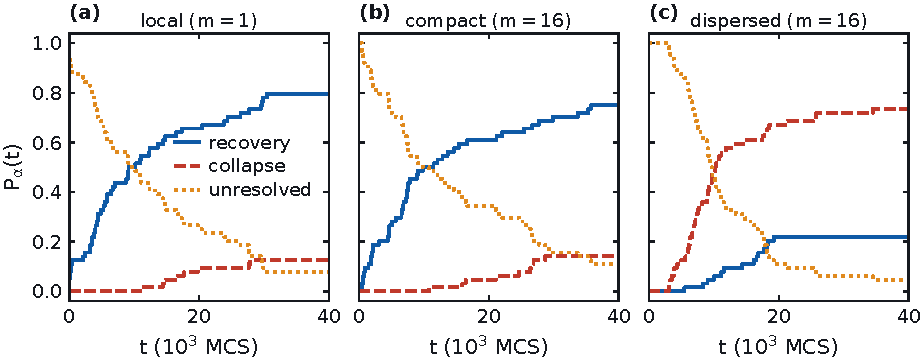
\includegraphics[width=0.85\textwidth]{fig03_fate_kinetics.pdf}
\caption{Outcome kinetics following (a) a single-site, (b) a compact 16-site, and (c) a dispersed 16-site perturbation. Each panel uses 64 independent realizations at the reference parameters. Recovery, collapse, and unresolved probabilities partition the full ensemble. Steps occur at recorded event times; the first event label is retained.}
\label{fig:kinetics}
\end{appendixfigure}



\begin{appendixfigure}
\centering
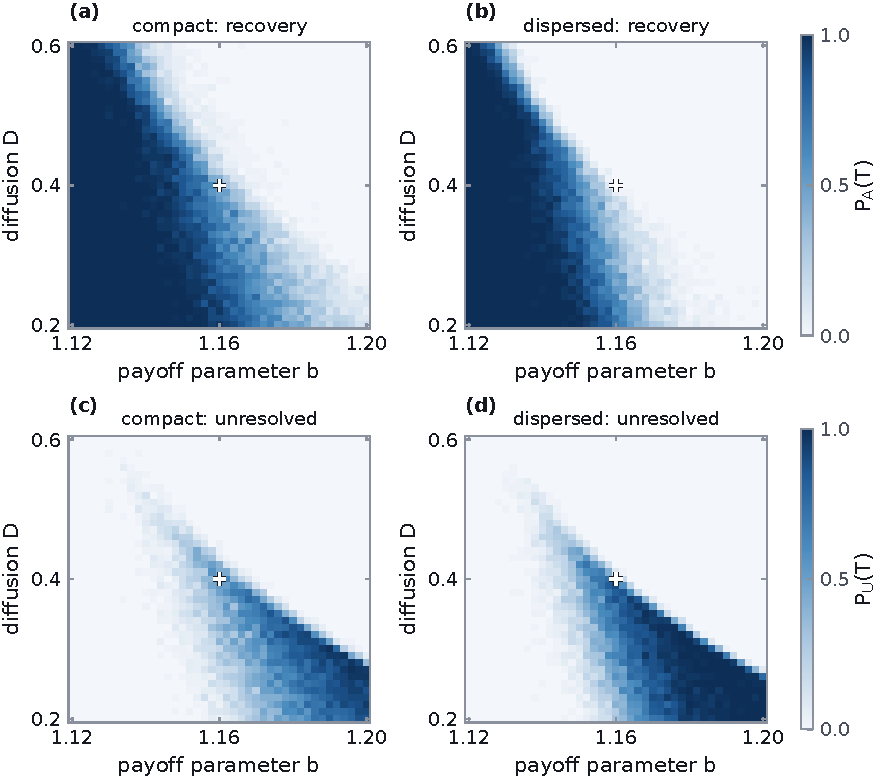
\includegraphics[width=0.8\textwidth]{figS01_recovery_unresolved.pdf}
\caption{Recovery (a,b) and unresolved (c,d) probabilities for compact and dispersed perturbations. Together with Fig.~\ref{main-fig:phase}, every parameter cell satisfies $P_A+P_B+P_U=1$ at $T=10000$ MCS. Crosses mark the reference parameters. Each cell contains 64 realizations per geometry; no interpolation is applied.}
\label{fig:outcomes}
\end{appendixfigure}

\end{minipage}

\clearpage
\noindent\begin{minipage}{\textwidth}

\begin{appendixfigure}
\centering
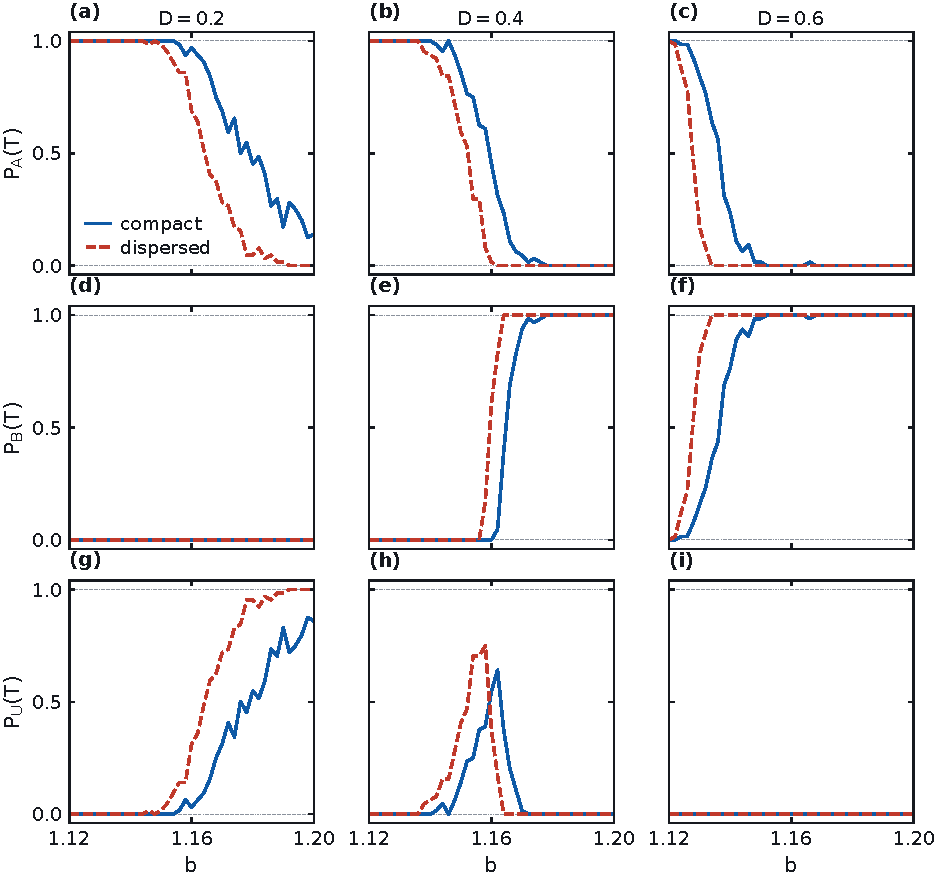
\includegraphics[width=0.8\textwidth]{fig05_phase_sections.pdf}
\caption{Competing outcomes along three diffusion sections. Columns show $D=0.2,0.4,0.6$; rows show recovery, collapse, and unresolved probabilities. Each panel compares the two geometries at all 41 measured payoff values, with 64 realizations per value and $T=10000$ MCS. Lines connect the sampled values. These sections distinguish transfer into unresolved evolution from transfer into collapse.}
\label{fig:sections}
\end{appendixfigure}



\begin{appendixfigure}
\centering
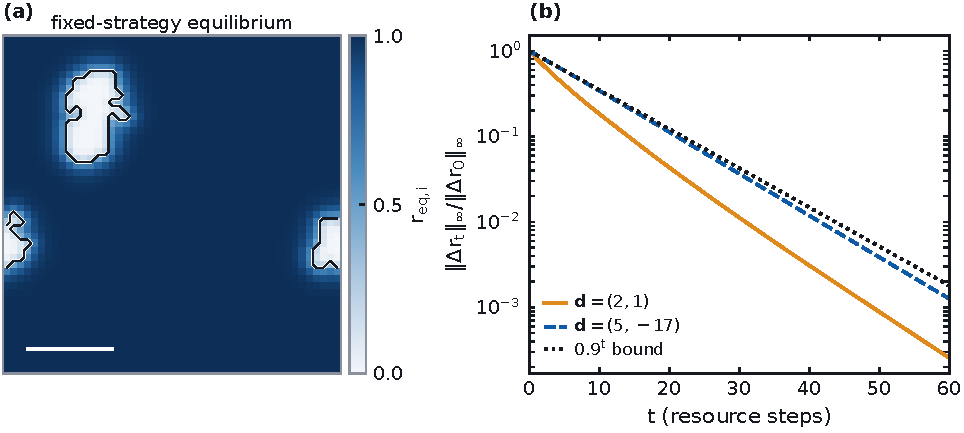
\includegraphics[width=0.8\textwidth]{figS06_resource_controls.pdf}
\caption{Resource adaptation at fixed strategies. (a) Equilibrium field for the strategy configuration in Fig.~\ref{main-fig:alignment}; scale bar: 12 sites. (b) Median normalized maximum-norm difference between translated and original fields over 48 configurations. The dotted curve is the contraction bound $0.9^t$. The strategy pattern is fixed throughout; this is not a relaxation-time measurement for the coupled system.}
\label{fig:resourcecontrols}
\end{appendixfigure}

\end{minipage}

\clearpage

\begin{appendixfigure}
\centering
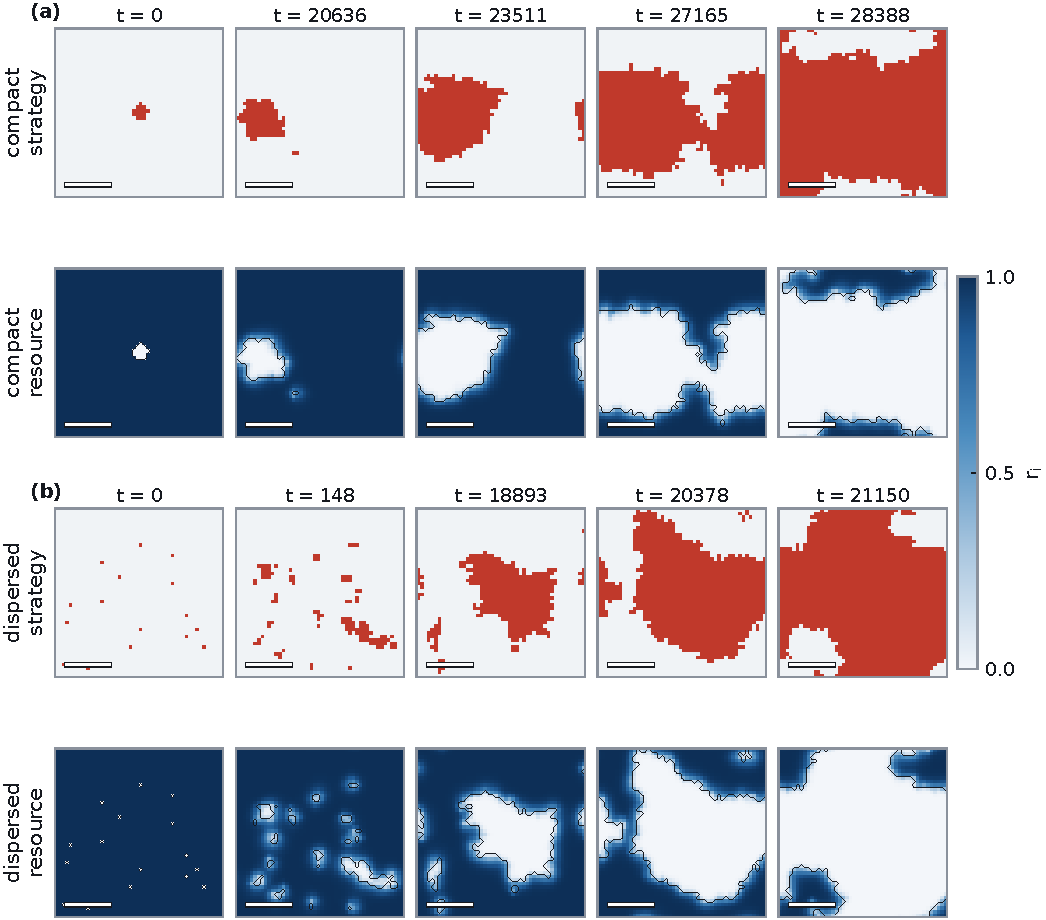
\includegraphics[width=0.87\textwidth]{figS03_full_growth_fields.pdf}
\caption{Strategy and resource evolution for the examples in Fig.~\ref{main-fig:fields}: (a) compact and (b) dispersed preparation. Columns show the initial state and first 5\%, 20\%, 50\%, and 80\% defector crossings. Red sites are defectors; resource maps share $0\le r_i\le1$. Time is in MCS and scale bars span 12 sites. Each trajectory uses one fixed spatial translation.}
\label{fig:fullfields}
\end{appendixfigure}


\clearpage
\noindent\begin{minipage}{\textwidth}

\begin{appendixfigure}
\centering
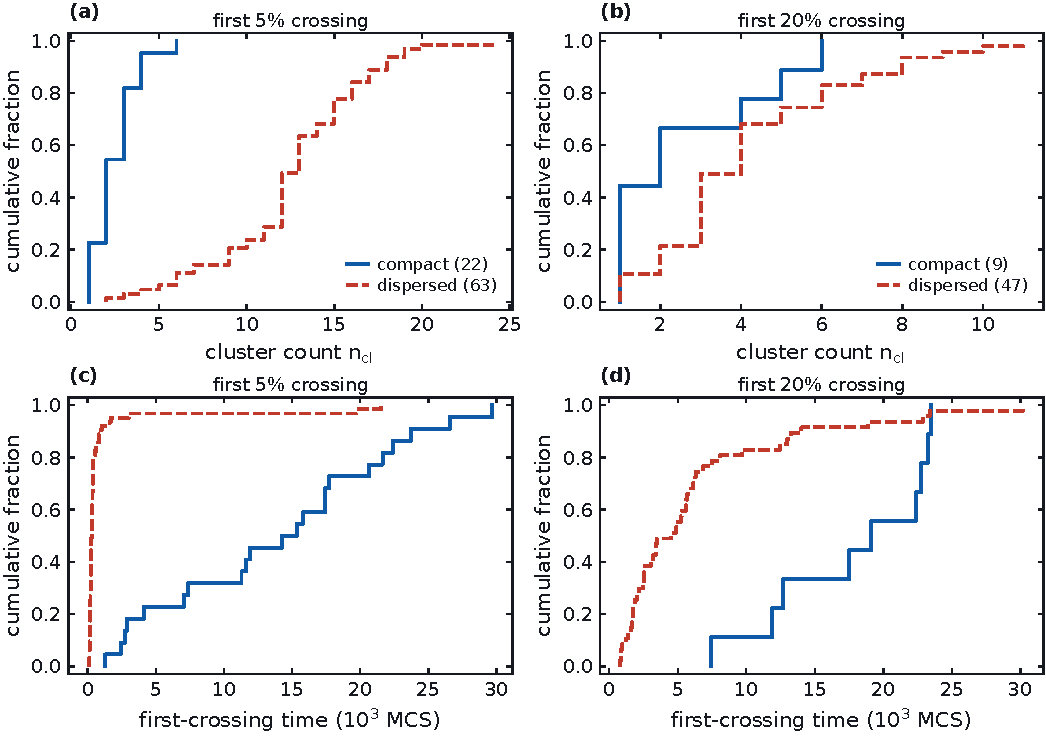
\includegraphics[width=0.8\textwidth]{figS04_growth_distributions.pdf}
\caption{Conditional spatial and first-passage distributions. (a,b) Periodic cluster counts at first 5\% and 20\% crossings. (c,d) Corresponding arrival times. Curves include every trajectory reaching the specified threshold by $T=40000$ MCS; legend counts give the denominators. The reaching subsets differ between geometries and thresholds.}
\label{fig:growthdistributions}
\end{appendixfigure}



\begin{appendixfigure}
\centering
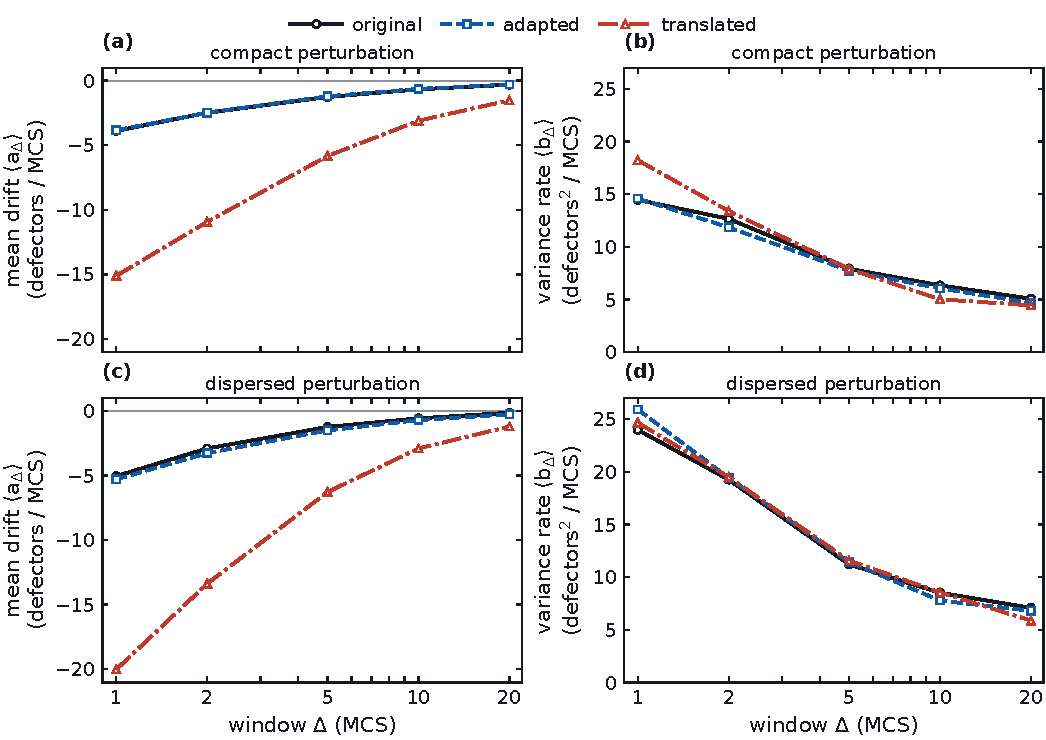
\includegraphics[width=0.8\textwidth]{fig06_conditional_moments.pdf}
\caption{Finite-window drift (left) and conditional variance rate (right) after resource redistribution. Rows distinguish compact and dispersed origins. Each mean uses 15 configurations at the first 5\% crossing and 64 continuations per configuration and treatment. Circles, squares, and triangles denote original, fixed-strategy-adapted, and translated $(17,12)$ fields. Lines join the five measured windows; these rates differ from the first-visit moments.}
\label{fig:windows}
\end{appendixfigure}

\end{minipage}

\clearpage

\begin{appendixfigure}
\centering
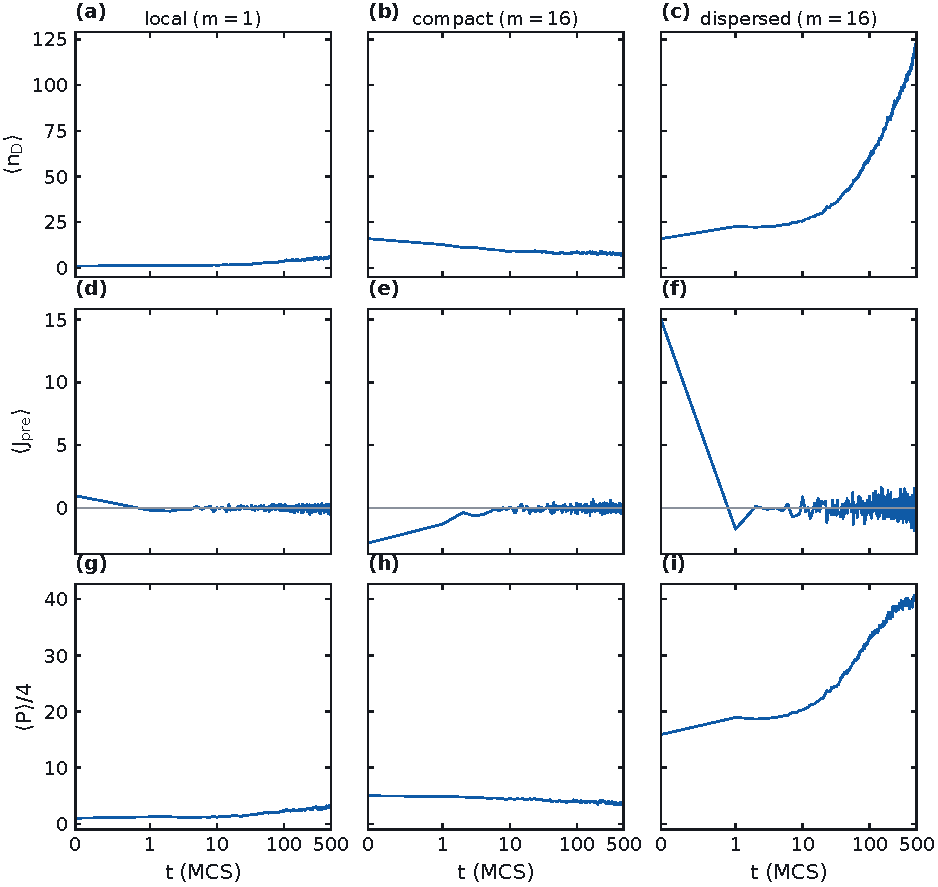
\includegraphics[width=0.86\textwidth]{fig04_interface_dynamics.pdf}
\caption{Early population growth, interface bias, and activity. Columns show single-site, compact, and dispersed preparations; rows show mean $n_D$, $J_{\rm pre}$, and $P/4$. Every recorded MCS through $t=500$ is included for all 64 realizations, including absorbed paths. Time is linear up to one MCS and logarithmic thereafter. The quantity $P/4=N\mathbb E[Z^2]$ measures frozen first-visit activity, not a complete-cycle variance.}
\label{fig:interface}
\end{appendixfigure}


\clearpage
\noindent\begin{minipage}{\textwidth}

\begin{appendixfigure}
\centering
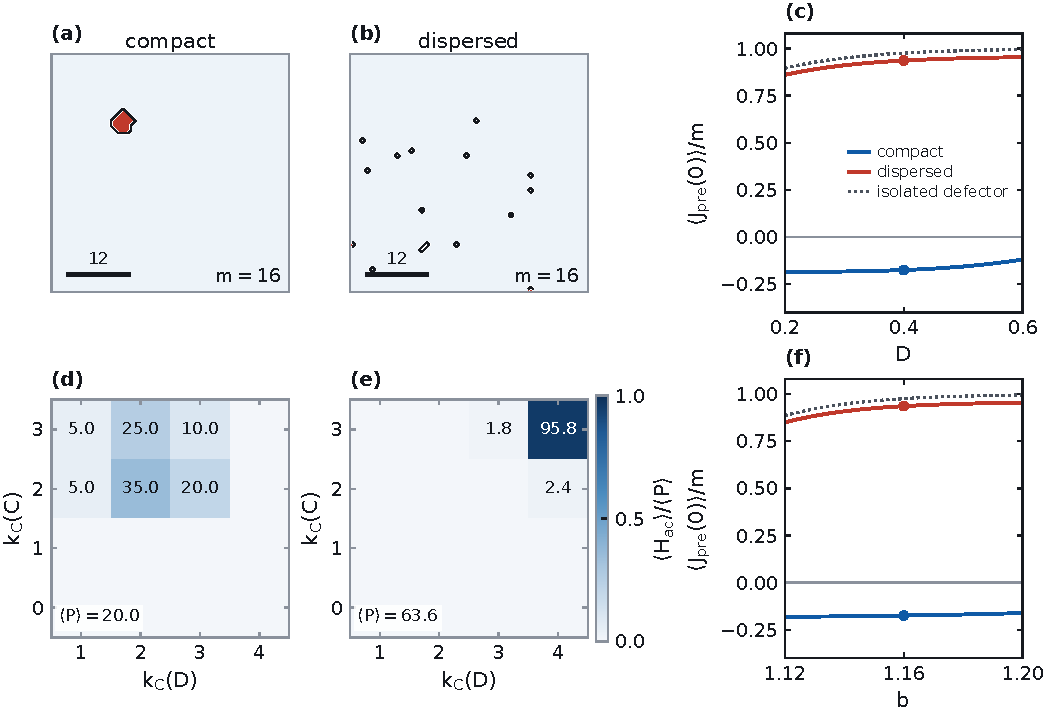
\includegraphics[width=0.84\textwidth]{fig09_initial_interfaces.pdf}
\caption{Initial interface geometry and growth bias. (a,b) Compact and dispersed 16-site preparations on the $48\times48$ lattice; red sites are defectors, pale-blue sites are cooperators, and bars span 12 sites. (c,f) Exact motif-based bias per initial defector as a function of $D$ at $b=1.16$ and of $b$ at $D=0.4$; dots mark the reference parameters and dotted curves show an isolated defector. These are frozen-initial-state diagnostics. (d,e) Fractions of interfacial edges with $a=k_C(C)$ and $c=k_C(D)$ cooperative neighbors. Numbers give percentages; the color scale is a fraction. Motifs and biases use all 64 preparations per geometry.}
\label{fig:initialinterfaces}
\end{appendixfigure}



\begin{appendixfigure}
\centering
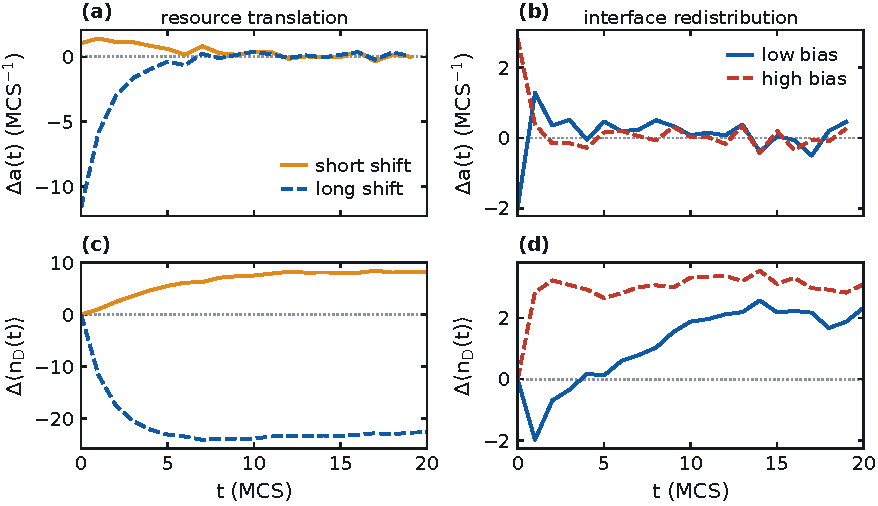
\includegraphics[width=0.8\textwidth]{fig07_cumulative_response.pdf}
\caption{Population response to translation (left) and boundary redistribution (right), relative to the original field. (a,b) Change in mean increment per MCS, $\Delta a(t)$. (c,d) Accumulated difference $\mathcal I_a(t)$. Means use 48 configurations and 16 continuations per treatment; translations average four rotations of $(2,1)$ (short) or $(5,-17)$ (long). Every recorded time through 20 MCS is shown.}
\label{fig:response}
\end{appendixfigure}

\end{minipage}

\clearpage

\begin{appendixfigure}
\centering
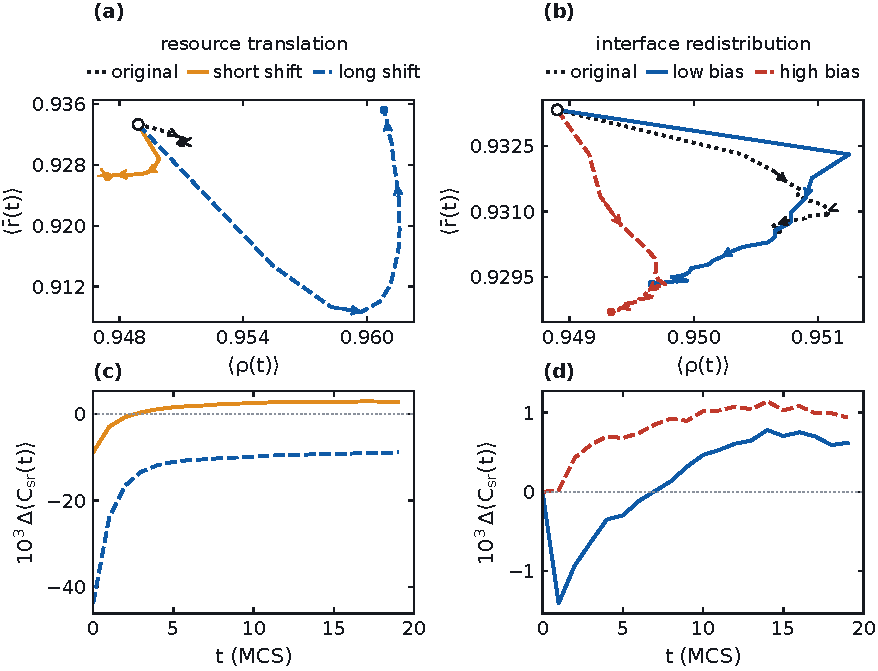
\includegraphics[width=0.8\textwidth]{fig08_coupled_response.pdf}
\caption{Coupled response of the ensembles in Fig.~\ref{fig:response}: translation (left), boundary redistribution (right). (a,b) Mean cooperation--resource paths over 20 MCS. Circles mark the common initial state (open) and endpoints (filled); arrows indicate increasing time. (c,d) Strategy--resource covariance changes, reconstructed per trajectory. These mean paths do not define a closed flow.}
\label{fig:feedback}
\end{appendixfigure}

\par

\bibliography{references}
\end{document}
